% !TEX TS-program = xelatex
% !TEX encoding = UTF-8
\documentclass[onecolumn,oneside]{SUSTechHomework}
\usepackage{graphicx}

\author{董骏博}
\sid{12432995}
\title{Homework 1}
\coursecode{CSE5001}
\coursename{Advanced Artificial Intelligence Fall 2024}

\begin{document}
    \maketitle
  
    \section*{Problem 1}
    \begin{figure}[h]
        \centering
        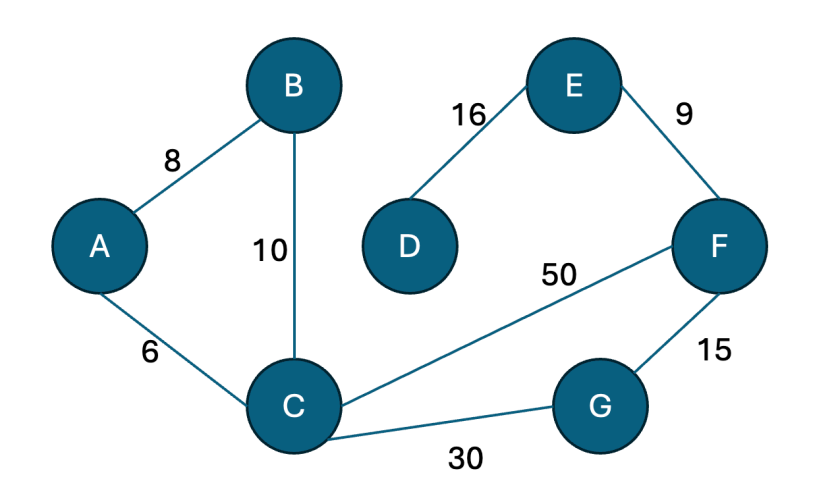
\includegraphics[width=0.6\textwidth]{task1.png} % 插入图片,设置宽度为文本宽度的一半
        % \caption{示例图片} % 图片的标题
        \label{fig:example} % 图片的标签,用于引用
    \end{figure}
    \subsection*{Task 1.1}
    由BFS算法,我们可以得到,从A点到D点的路径为:\textbf{A, C, F, E, D},\[\text{cost} = 6 + 50 + 9 + 16 = 81 \]
    \subsection*{Task 1.2}
    由DFS算法可得,从A点到D点的路径为:\textbf{A, C, G, F, E, D},\[\text{cost} = 6 + 30 + 15 + 9 + 16 = 76 \]
    \subsection*{Task 1.3}
    由UCS算法可得,从A点到D点的路径为:\textbf{A, C, G, F, E, D},\[\text{cost} = 6 + 30 + 15 + 9 + 16 = 76 \]
    \newpage
    \section*{Problem 2}
    \begin{figure}[h]
        \centering
        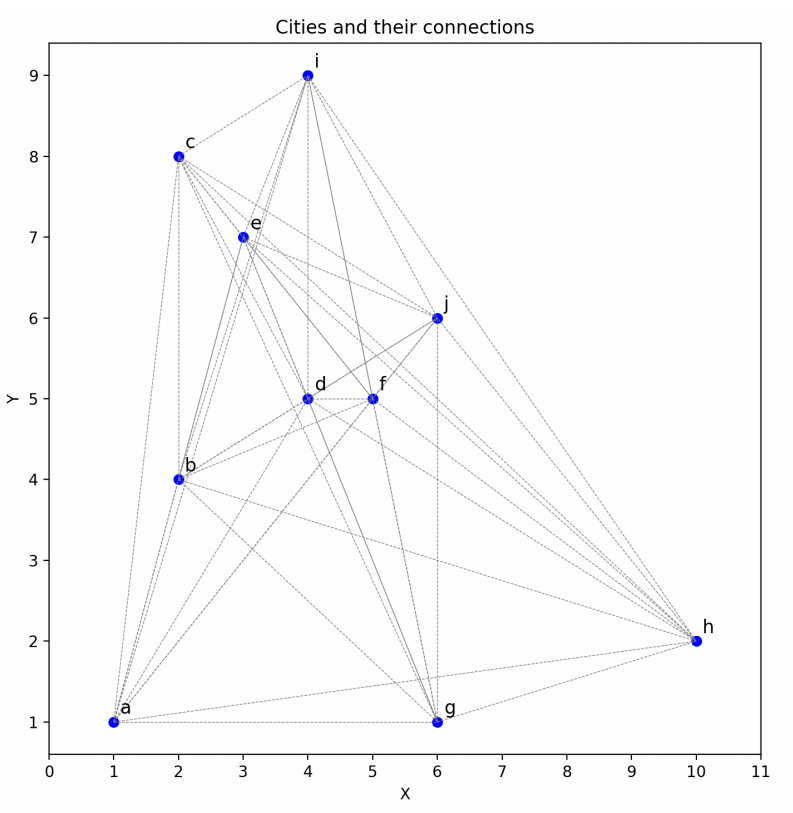
\includegraphics[width=0.6\textwidth]{task2.png} % 插入图片,设置宽度为文本宽度的一半
        % \caption{示例图片} % 图片的标题
        \label{fig:example} % 图片的标签,用于引用
    \end{figure}
    \subsection*{Task 2.1}
    
\end{document}